\documentclass[brazil]{abnt}
\usepackage[utf8]{inputenc}
\usepackage[brazil]{babel}
\usepackage{listings}

\usepackage{courier}
 \lstset{
         basicstyle=\footnotesize\ttfamily, 
         numberstyle=\tiny,          
         numbersep=5pt,              
         tabsize=2,                  
         extendedchars=true,         
         breaklines=true,            
         keywordstyle=\color{red},
                frame=b,         
         stringstyle=\color{white}\ttfamily, 
         showspaces=false,           
         showtabs=false,             
         %xleftmargin=17pt,
         %framexleftmargin=17pt,
         %framexrightmargin=5pt,
         %framexbottommargin=4pt,
         %backgroundcolor=\color{lightgray},
         showstringspaces=false      
 }
 \lstloadlanguages{
         %[Visual]Basic
         %Pascal
         %C
         C++
         %XML
         %HTML
         %Java
 }

\usepackage{color}
\usepackage{xcolor}
\usepackage{graphicx}
\usepackage{wrapfig}
\usepackage{xunxos-utp}
\usepackage{caption}
\DeclareCaptionFont{white}{\color{white}}
\DeclareCaptionFormat{listing}{\colorbox{gray}{\parbox{0.98\textwidth}{#1#2#3}}}
\captionsetup[lstlisting]{format=listing,labelfont=white,textfont=white}


\makeatletter
\usepackage{babel}
\makeatother
\begin{document}

\autor{Renato dos Santos Cerqueira}
\coautor{Felipe Pedrosa Martinez}
\titulo{Title Placeholder}
\orientador{Adriano Joaquim de Oliveira Cruz}
\comentario{Monografia apresentada para obtenção do Grau de Bacharel em Ciência da Computação pela Universidade 
Federal do Rio de Janeiro.}
\instituicao{Departamento de Ciência da Computação \par Instituto de Matemática \par Universidade Federal do Rio de Janeiro}
\local{Rio de Janeiro - RJ, Brasil}
\data{21/12/2012}

\Ncapa
\NFolhaDeRosto

\begin{folhadeaprovacao}
Monografia de Projeto Final de Graduação sob o título \textit{``\ABNTtitulodata''},
defendida por \ABNTautordata~e \ABNTcoautordata~e aprovada em \ABNTdatadata, no Rio de Janeiro,
Estado do Rio de Janeiro, pela banca examinadora constituída pelos
professores: \setlength{\ABNTsignthickness}{0.4pt}

\assinatura{Prof. Ph.D. Adriano Joaquim de Oliveira Cruz\\ Orientador} \assinatura{???\\ Universidade ???} \assinatura{???\\ Universidade ???}
\end{folhadeaprovacao}

\begin{resumo}
O objetivo deste trabalho é fazer um \textit{engine} de jogo para o \textit{videogame Nintendo DS\texttrademark} e também um editor de fases 
e configurações, como seria feito numa equipe de desenvolvimento de um jogo comercial, dando a possibilidade aos \textit{designers} 
de fazerem seus \textit{sprites} e criarem as fases com eles, sem que fosse necessário mexer com códigos.
\end{resumo}

\begin{abstract}
The objective of this paper is to make a game engine to the Nintendo DS\texttrademark system and a level and configurations editor, as it
would be done in a development team in a comercial game, giving designers the possibility to make their sprites and create their levels 
without touching actual source code.
\end{abstract}

\chapter*{Dedicatória}

\chapter*{Agradecimentos}

\tableofcontents{}
\listoffigures
\listoftables

\chapter{Introdução\label{cap:introducao}}

\vfill{}
\begin{flushright}{}``\emph{Quote 1}''\\
{\small Author1}\end{flushright}{\small \par}
\vfill{}

Neste capítulo são apresentados o objetivo desta monografia e a estrutura
da mesma.
\newpage


\section{Objetivo deste trabalho}

A área de jogos eletrônicos é uma área relativamente nova, se comparada a outros ramos da ciência da computação. No entanto, por mais que compreenda conceitos importantes de computação, engloba outros que fogem ao seu escopo. Para o desenvolvimento de um jogo eletrônico, além de conhecimentos de linguagens de programação, algoritmos e estruturas de dados, interface humano-computador, inteligência artifical, etc; é preciso considerar aspectos mais subjetivos que dizem respeito a um jogo de forma geral, seja ele eletrônico ou não. O gameplay, ou a mecânica do jogo, ou seja, a forma com que o jogo vai se desenrolar e o seu funcionamento, é um exemplo claro de que o seu desenvolvimento e sua concepção vão muito além do que pode ser programado, compilado e executado em um computador.

É possível observar o crescimento da área se notarmos que o primeiro exemplo conhecido de jogo eletrônico aparece em 1947, quando Thomas T. Goldsmith Jr. e Estle Ray Mann introduziram sua patente para um Dispositivo de Entretenimento usando Tubo de Raios Catódicos em \\\cite{2455992}. Jogos produzidos na época do Atari 2600 e Magnavox Odyssey, por exemplo, eram criações de um único desenvolvedor e em geral, desenvolvidos em períodos curtos de tempo, sem nem ao menos identificar o time de desenvolvimento. Era comum a aparição de \textit{Easter Eggs}, recursos que os desenvolvedores usavam para identificar a sua criação, mesmo que de uma forma não convencional \cite{PrimeiroDevName}.

Com a tecnologia cada vez mais aprimorada, conceitos básicos que definiam os jogos daquela época vêm sido substituídos por formas cada vez mais rebuscadas. Novos elementos de jogabilidade vêm sido incorporados à mecânicas clássicas, e estas evoluem por si só, dadas as cada vez menores limitações e as constantes inovações de hardware e interação com o jogador. Isso tudo se reflete no desenvolvimento de novas áreas de jogos: onde antes haviam poucos estilos bem definidos, como corrida, luta e aventura, encontramos novos nichos como por exemplo jogos casuais, sociais e de multiplay massivo.

Hoje em dia, a indústria de jogos conta com super~produções com uma quantidade quase infindável de desenvolvedores, designers, criadores de fases, dentre outros tantos profissionais trabalhando cada um com sua especialidade.

Neste trabalho, o que nos propomos a fazer é nos inserir no contexto desses times de criação modernos, vendo apenas uma pequena parte dessa grande cadeia de desenvolvimento: a criação de ferramentas para facilitar a interação entre equipes de ramos diferentes. Mais especificamente, criando um jogo em duas dimensões, do tipo plataforma para o videogame portátil Nintendo DS. Para isso, desenvolvemos uma engine, responsável por controlar todas as partes envolvidas no funcionamento do jogo como áudio, vídeo, estruturas de dados, controle de personagens, fases, itens etc. Parte do nosso objetivo foi tornar esta engine  simples e de fácil reutilização. Isto foi feito através de ferramentas de criação e configuração dos componentes pertinentes ao mundo do jogo.

Nos propomos a fazer o papel do desenvolvedor: Criar as ferramentas, imaginando como os outros times as usariam e aprimorando-as ao máximo para esse fim.

\section{Contextualização}

Nos propomos a criar ferramentas para desenvolver jogos em duas dimensões do tipo de plataforma. O questionamento imediato a partir desta proposta é: o que é exatamente um jogo de plataforma em duas dimensões? Basicamente, são jogos onde a movimentação do personagem principal se dá verticalmente ou horizontalmente, sem considerar a aproximação ou o distanciamento deste ao jogador. Conforme o personagem se desloca pelo mundo, este vai se revelando a ele, e é comum que apresente inimigos e obstáculos, como uma fileira de espinhos ou buracos sem fundo. Em geral, o personagem principal tem um objetivo que o motiva a atravessar o mundo que o é apresentado, podendo ou não saltar ou possuir alguma habilidade especial, ter ou não acesso a alguma arma ou item, e enfrentar algum grande inimigo no final de tudo. Esta é uma definição bastante aberta, e é nela que nos inspiramos para escrever o motor que será executado no Nintendo DS. Para ilustrar, podemos pensar em exemplos clássicos, como Super Mario World para o Super Nintendo, ou Sonic The Hedgehog para o Sega Mega Drive.

Nem todos os jogos plataforma são em duas dimensões. Entretanto, vamos aqui nos focar neles para facilitar o entendimento e o desenvolvimento de soluções. Nessa modalidade, uma característica comum presente em muitos jogos é o uso de \textit{tiles}, figuras de tamanho pré-definido, que compõem todo o mundo. \textit{Tile}, em inglês, significa ladrilho. Além disso, nesse tipo de jogo, todos os objetos costumam ser feitos da combinações de \textit{sprites}, usados mais de uma vez e em diferentes posições. Os \textit{sprites} são responsáveis por representar possiveis inimigos, por exemplo. Para simplificar, é possível se dizer que enquanto os \textit{tiles} compõem o mundo, os \textit{sprites} o habitam.

Nosso objetivo é criar uma engine que leia um arquivo de configuração, onde estarão detalhadas informações sobre quais são as imagens que compõem o personagem principal (ou personagens, no caso de haver uma escolha); informações sobre os inimigos como por exemplo a qual tipo de movimento que cada um obedece; descrição dos itens, como por exemplo qual efeito ele causa no personagem principal ou nos inimigos e informações sobre as fases, dentre elas o posicionamento dos elementos que as compõem.

\section{Estrutura da monografia}

Escrever aqui a estrutura da monografia.

\chapter{Desenvolvendo para o Nintendo DS\label{cap:hardds}}

\vfill{}
\begin{flushright}{}``\emph{Quote 2}''\\
{\small Author 2}\end{flushright}{\small \par}
\vfill{}

Neste capítulo são apresentados a motivação para desenvolver para a plataforma, as suas especificações e como desenvolver.
\newpage

\section{Motivação}

Há poucos trabalhos desenvolvidos para plataformas diferentes do PC, seja pelo mais restrito número de usuários, menor versatilidade de ferramentas e recursos associados ou mesmo pela maior dificuldade de encontrar documentação relativa ao desenvolvimento. A motivação para este trabalho é, dada essas circunstâncias, criar um facilitador para o desenvolvimento de jogos para um console real, desenvolvendo ferramentas para fomentar uma maior quantidade de trabalhos para a plataforma, apesar das dificuldades.

\section{Especificações}

O foco deste trabalho se dá nas duas primeiras iterações do Nintendo DS: o Nintendo DS original, lançado no final de 2004, que normalmente é chamado de ``DS Phat''; e sua segunda iteração, o Nintendo DS Lite, lançado no meio de 2006.

Ambos possuem um hardware muito parecido, sendo as suas maiores diferenças são a estética e o contraste e iluminação da tela. Nesta seção, são detalhadas as especificações de cada um:

\noindent{\bf Nintendo DS:}\\
{\bf Peso:} 275 gramas\\
{\bf Dimensões:} 148.7mm x 84.7mm x 28.9mm\\
{\bf Telas:} Duas telas, ambas com 3 polegadas, de LCD TFT (Thin-Film Transistor) com 18-bit de cor, resolução de 256x192. As duas telas tem um espaço entre elas de aproximadamente 21mm. A tela inferior possui \textit{touchscreen} resistivo, que responde a um ponto de pressão por vez. No caso de vários pontos da tela serem pressionados simultaneamente, ela responde na posição média destes pontos.\\
Além disso, a tela possui iluminação traseira, que pode ser desligada por software.\\
{\bf Entradas:} Duas entradas de cartucho, uma para o formato de cartucho do seu antecessor, o Gameboy Advance(GBA), na parte inferior,e uma para seu próprio formato de cartucho na parte superior.\\
{\bf Processadores:} Dois processadores ARM, um ARM946E-S a 67MHz, que é o processador principal, responsável pelo loop de jogo e renderização de vídeo e um coprocessador ARM7TDMI a 33MHz, responsável pelo som, wi-fi, e que quando em modo GBA, diminui seu clock para 16MHz, e passa a ser responsável pelo processamento principal.\\
{\bf Memória:} 4MiB de RAM principal, expansíveis através da entrada de Gameboy Advance. No entanto, essa expansão só foi usada em jogos oficiais pelo Opera Browser.\\
{\bf Wireless:} Conexão IEEE802.11b, compatível com encriptação por WEP. WPA e WPA2 não são suportadas. Essa conexão também pode ser usada para comunicação entre consoles.\\

\noindent{\bf Nintendo DS Lite:}\\
{\bf Peso:} 218 gramas\\
{\bf Dimensões:} 133mm x 73.9mm x 21.87mm\\
{\bf Telas:} Mesma especificação que o original, no entanto, possui quatro níveis de iluminação que podem ser reguladas por software. A tela também possui um contraste melhor que o original.\\
Existem algumas outras menores diferenças, como a mudança do chip que controla o Wireless, o controlador da \textit{touchscreen} também é ligeiramente diferente, mas para fins práticos, o resto da configuração é igual ao original.

\section{Desenvolvimento}

O desenvolvimento oficial no DS segue os mesmos moldes do desenvolvimento em consoles diversos: a Nintendo possui um time interno chamado de Intelligent Systems Co. Ltd. responsável pelas ferramentas de desenvolvimento para os consoles da empresa, dentre eles, o Nintendo DS. O desenvolvedor interessado pode entrar em contato em busca das ferramentas para tal, que incluem uma unidade especial conectada ao computador por meio de uma porta USB. Dentre outras particularidades, esta unidade possui o dobro de memória de uma unidade normal, de forma a facilitar o Debug. No entanto, para adquiri-las, é necessário assinar um Acordo de Confidencialidade (do inglês, Non-Disclosure Agreement), que não permite que se comente ou escreva sobre esses kits de desenvolvimento. Por causa disto, é difícil encontrar mais detalhes acerca de seu funcionamento.

\begin{figure}
\centering
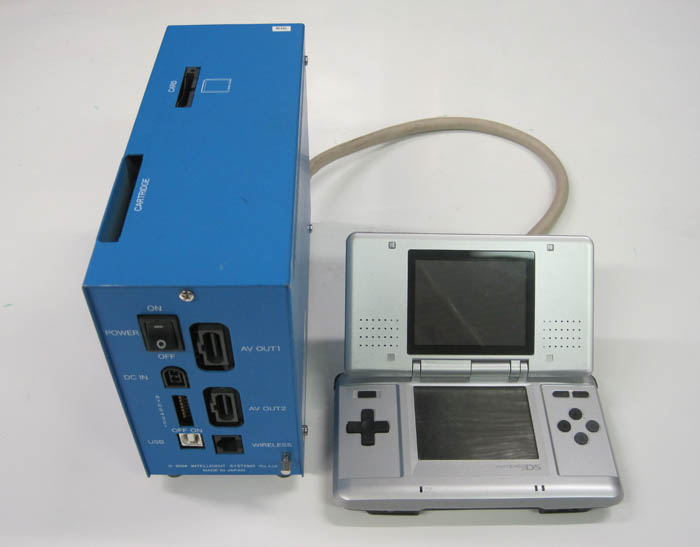
\includegraphics{imgs/is_devkit1.jpg}
\caption{Uma imagem do kit de desenvolvimento oficial do Nintendo DS original} 
\end{figure}

Em geral, pequenas empresas de desenvolvimento não têm acesso ao kit de desenvolvimento oficial, seja por causa dos altos custos para adquirir o hardware ou pela dificuldade de adquirir as licenças. Desta forma, a publicação de jogos para consoles do tipo ainda é rara no mercado atual de jogos.

Para nós, cabe recorrer ao desenvolvimento não oficial, apelidado de Homebrew. A cadeia de ferramentas usada é chamada devkitArm, que serve para compilar programas em C e C++ para consoles com processadores ARM. Ao contrário do desenvolvimento oficial, não é possível produzir cartuchos de jogos Homebrew. Para testarmos, no entanto, podemos fazer uso de emuladores ou de um Nintendo DS com uso de um flash cartridge, um cartucho que possui uma memória flash, como um pendrive, e que pode ser apagada e reescrita várias vezes. Este cartucho não é suportado pela Nintendo.

A partir do devkitArm, foi desenvolvida a libnds, feita especificamente para o hardware do DS. Essa biblioteca inclui funções de baixo nível que acessam todo o hardware: som, video, wireless, controle, dentre outros. O desenvolvimento nela apresenta dificuldades dado o baixo nível de suas instruções. Muitas vezes é necessário o uso de endereços de memória, cópias diretas da memória principal para a memória de vídeo, dentre outros artifícios não usuais na programação atual. Dado este cenário, baseadas na libnds, surgiram algumas bibliotecas em um nível mais alto.

Para o desenvolvimento deste trabalho, foi escolhida a PALib, uma biblioteca que visa facilitar o desenvolvimento de jogos em duas dimensões que usem \textit{sprites} e mapas de fundo.

Ainda assim, o uso dessas ferramentas não é trivial. Diferente de um programa convencional para desktop, as suas funcionalidades se apresentam em formas menos claras para o desenvolvedor: incluir ou gerar imagens, por exemplo, implica em um fluxo de trabalho diferente do esperado por um time de desenvolvimento convencional. 

O conjunto de ferramentas desenvolvidos neste trabalho tem como objetivo tornar mais transparente e intuitivo o desenvolvimento no cenário apresentado. As ferramentas desenvolvidas são, em sua maioria, visuais para que o seu uso se dê de uma forma simplificada.

% escrevi esse parágrafo sobre QT, mas ele provavelmente precisa de uma revisada.

Para desenvolver as ferramentas foi usado o QT, um \textit{Framework} multi-plataforma que permite o uso de interfaces gráficas em C++, além de ter classes que facilitam o acesso a tecnologias como XML, acesso a diversos formatos de arquivos de imagem, dentre outras possibilidades. A escolha foi feita para que as ferramentas funcionem em diversos sistemas operacionais sem precisar de mudanças no código.

\chapter{As ferramentas\label{cap:ferramentas}}

\vfill{}
\begin{flushright}{}``\emph{Quote 3}''\\
{\small Author 3}\end{flushright}{\small \par}
\vfill{}

Neste capítulo são apresentadas as ferramentas e o seu método de uso.
\newpage

\section{A criação do jogo\label{sec:workflow}}

Um jogo necessita de algumas partes constituintes, como por exemplo, suas fases e cenários, seus itens, inimigos e personagem principal. Com o uso das ferramentas apresentadas neste trabalho, o usuário executa os seguintes passos:

Em primeiro lugar, o usuário cria os cenários usando a BGTool, onde ele desenha os cenários em que o jogo vai se passar. Esses cenários ficam organizados logicamente em fases, e essas fases no produto final aparecerão encadeadas.

Em seguida, é necessário importar as figuras dos personagens, inimigos e itens. Isso é feito a partir da SpriteTool. 
%\footnote{Precisamos pensar em como juntar as duas coisas. Como o usuário posiciona inimigos e itens no cenário? Há uma terceira ferramenta? Fazemos uma das duas ferramentas fazerem isso, adicionalmente?}

\section{BGTool: A ferramenta de criação de cenários}

A BGTool foi criada com o objetivo de permitir que o usuário importe seus tiles pré-existentes e a partir deles, desenvolva um novo cenário e consiga exportar esse cenário para o formato do Nintendo DS. 

Ao começar um novo projeto, o usuário pode escolher quantas camadas de \textit{background} o cenário sendo criado terá. O hardware do DS suporta até cinco camadas de \textit{background}, no entanto, é possível o uso de menos camadas do que isso. Com as várias camadas, porém, o usuário pode criar uma ilusão de movimento em profundidades diferentes, um recurso conhecido como rolamento em paralaxe.\footnotemark

\footnotetext{Rolamento em Paralaxe é uma técnica em que as camadas mais distantes da câmera se movem mais devagar, dando uma ilusão de profundidade e imersão.}

Por uma combinação do hardware do DS e das bibliotecas usadas, uma camada de \textit{background} na verdade é um mapa de \textit{tiles}. Isto quer dizer que as imagens são compostas de imagens menores, de tamanho fixo, que podem ou não ser rotacionadas ou espelhadas na vertical ou horizontal. E estas imagens menores são chamadas de \textit{tiles}, como mostramos anteriormente.

Portanto, além do número de camadas, o usuário também especifica o tamanho dessas. A única limitação quanto ao seu tamanho é ter suas dimensões múltiplas de 8, isto quer dizer que usamos \textit{tiles} de tamanho 8x8, o mais simples de ser utilizado no DS.

\begin{figure}[h!]
\centering
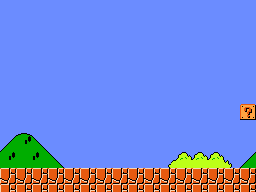
\includegraphics[scale=1]{imgs/exemplo.png}
\caption{A imagem antes de ser carregada} 
\end{figure}

\begin{figure}[h!]
\centering
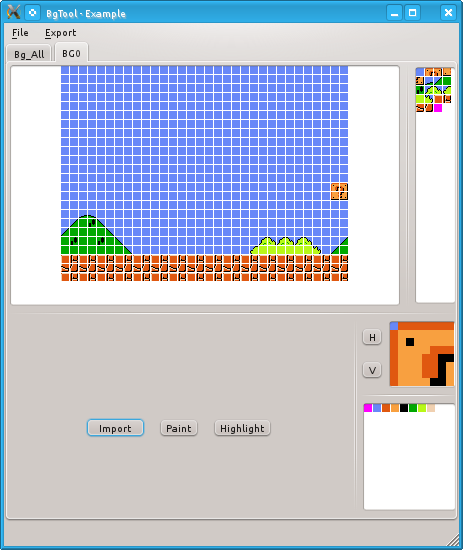
\includegraphics[scale=1]{imgs/bgtool1.png}
\caption{A imagem após a abertura na ferramenta} 
\end{figure}

Ao importar os tiles, o usuário pode usá-los para editar o mapa dos cenários. Uma paleta é gerada automaticamente pela ferramenta a partir dos tiles que o usuário carrega. A ferramenta se encarrega de fazer a importação de uma imagem e transformá-la em tiles, dividindo a imagem em partes de 8x8 e eliminando as partes que são iguais. Como o DS suporta espelhamento na horizontal e na vertical de um tile, verificamos então se o tile em questão sendo avaliado é igual a um dos tiles existentes em quaisquer das configurações: sem espelhamento, com espelhamento vertical, horizontal ou ambos.

Como armazenamos os \textit{tiles} como uma imagem, não há um algoritmo de hash para essa imagem disponível no QT, por isso, fazemos uma busca pelo vetor de imagens comparando, manualmente, as imagens geradas com as imagens que já existem. Embora esse seja um processo relativamente custoso, com O(n) para cada inserção, ignoramos por ora esse custo.

\begin{figure}[h!]
\centering

\includegraphics[scale=1]{imgs/tiles1.png}
\caption{Alguns \textit{tiles} depois de separados} 
\end{figure}

\begin{figure}[h!]
\centering

\includegraphics[scale=1]{imgs/tiles2.png}
\caption{Configurações possíveis para um \textit{tile}} 
\end{figure}

Com os tiles já importados, o usuário pode então construir os mapas que compõem a fase nas abas relativas as várias camadas, e ter uma idéia de como ficará a versão final a partir da aba que mostra a composição das abas existentes.

O projeto pode ser salvo, nesse caso, guardamos o projeto num arquivo XML com um formato delimitado para que suporte todas as ferramentas. A BGTool guarda suas informações num nó BGTool abaixo do nó raiz do documento do projeto. Lá, ficam organizadas suas informações das diversas fases e camadas em cada fase. Isso será explicado com mais detalhes na seção \ref{sec:xml}.

A qualquer momento, o usuário pode exportar o que já está pronto para o DS, esse é um processo transparente em que criamos os arquivos necessários para a execução da fase criada pelo usuário. São criados três arquivos, um arquivo Pal, que contém a paleta, um arquivo Tile que contém os tiles, indexados pela paleta e um arquivo Map, que contém o mapa, indexado pelos tiles.

Todos os três arquivos são binários e obedecem a um formato delimitado pela PALib e suas funções que coordenam o carregamento de cenários.

Uma breve explicação desses formatos é a seguinte:

\begin{itemize}
 \item Arquivo Pal\\
 Neste arquivo, temos informações sobre a paleta usada no arquivo. São descritas todas as cores contidas no arquivo. Precisam haver 256 cores, mesmo que o arquivo seja inflado de cores falsas. O Formato usado no arquivo é A1B5G5R5, o que significa que há um bit para o caso da cor ser transparente (alpha channel), 5 para o verde, 5 para o azul e 5 para o vermelho. A primeira cor no arquivo é a cor usada como transparência. (A cor padrão sendo o Magenta)\label{exp:A1B5G5R5}
 \item Arquivo Tiles\\
 Neste arquivo, ficam os tiles, cada um de 8x8 pixels. Cada pixel do tile referencia uma cor do arquivo Pal. Neste arquivo, os tiles são escritos em blocos (vetores) de 64 bits. 
 \item Arquivo Map\\
 Neste arquivo, fica o mapa do \textit{background}, ele referencia os tiles. Os bits 0-9 indicam o tile, o bit 10 indica se é espelhado na horizontal e o bit 11 indica se é espelhado na vertical. Os bits restantes indicam qual paleta está sendo usada para o mapa em questão, eles não são usados nos modos em que só há uma paleta, ou seja, modos de 256 cores.
 \item Arquivo .c\\
 Este arquivo constrói a struct que será usada no programa, informa algumas coisas como o tipo do mapa, o seu tamanho, os ponteiros para as regiões onde ficaram os três arquivos acima depois de linkados, tamanho do tiles em bytes e tamanho do map em bytes. 
\end{itemize}

A conversão do arquivo de imagem é feita quando o usuário carrega uma nova imagem. Essa imagem é convertida para uma imagem de 256 cores. Idealmente, devido as diferenças de cor, a sugestão é que o usuário já carregue imagens limitada a 256 cores para evitar perda e caso carregue mais uma imagem, isto é, mais um conjunto de \textit{tiles} que estas tenham a mesma paleta.

Depois dessa conversão inicial, todas as ações no programa são feitas usando a paleta gerada na fase de carregamento. Na exportação, a paleta é exportada diretamente, simplesmente a colocamos para o arquivo binário.

Os tiles, quando exportados, também não necessitam de preocupação adicional. Sua conversão para o formato binário apenas envolve obter o indice da cor de cada pixel de cada tile e escrevê-lo no arquivo binário.

A geração do mapa é a tarefa mais complexa. Internamente na ferramenta, armazenamos o mapa como uma matriz de estruturas do tamanho do cenário, onde a estrutura armazena o indice do tile daquela posição e também se naquela posição este tile está espelhado na vertical, na horizontal ou ambos. Então obtemos essa transformação e jogamos para o formato discutido acima e exportamos para o arquivo binário.

Por fim, depois de exportados, esses arquivos estarão prontos para serem usados num estágio posterior e inseridos no jogo final.

\section{SpriteTool: A ferramenta de criação de sprites}

A SpriteTool foi criada com o objetivo de a partir de simples imagens, gerar \textit{sprites} para o desenvolvimento de um jogo completo executável no Nintendo DS. O objetivo da ferramenta é criar um ambiente para o usuário, no qual ele não tenha que lidar com particularidades do desenvolvimento que não sejam pertinentes a criação do \textit{sprite} em si.

Além de permitir a portabilidade das imagens para o Nintendo DS, transformando-as em \textit{sprites} do jogo no formato reconhecido pelo console, a SpriteTool gera um arquivo de projeto no formato XML, que pode ser reconhecido pelas outras ferramentas desenvolvidas neste trabalho. A integração entre estas ferramentas é feita respeitando protocolos pré-estabelecidos de escrita e leitura nestes arquivos, de forma transparente para o usuário. A seção \ref{sec:xml} aborda em detalhes a estrutura do formato escolhido e como cada uma das ferramentas faz uso dele para armazenar e resgatar as informações pertinentes ao desenvolvimento do jogo.

\begin{figure}[h!]
\centering
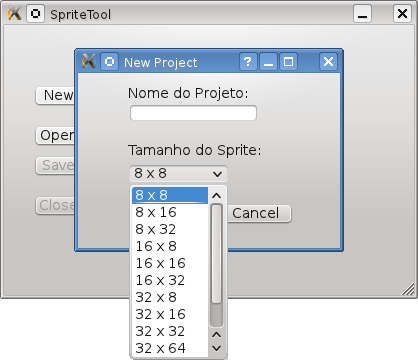
\includegraphics{imgs/spritetool1.png}
\caption{Janela de criação de novo \textit{sprite}} 
\end{figure}

Ao começar um novo projeto, uma instância de \textit{sprite} é criada, mesmo que ainda não tenha sido adicionada nenhuma imagem. É importante salientar que o termo “Sprite” neste escopo, engloba uma série de conceitos que vão além de um simples arquivo de imagem. São eles: informações relativas ao tamanho da imagem, uma paleta de cores, informações sobre transparência e enfim os frames do \textit{sprite} – que são as imagens em si.
Algumas destas informações são requeridas para a criação do projeto de \textit{sprite}, como o nome do \textit{sprite} e as dimensões das imagens que servirão como frames da animação deste. O programa oferece uma gama de formatos de \textit{sprite} para o usuário escolher, respeitando as restrições das bibliotecas e do hardware do DS sobre as imagens que podem ser usadas como \textit{sprites}.

Criado um novo projeto de \textit{sprite}, o usuário tem a possibilidade de adicionar novas imagens a ele. Além de permitir que o usuário busque uma imagem compatível com o tamanho já definido, o programa cria uma pasta de projeto e mantém nesta pasta uma cópia de cada imagem adicionada a ele, eliminando o uso de caminhos específicos para os arquivos fontes das imagens selecionadas. Assim, o programa tem uma maior portabilidade de uso. De forma análoga, as imagens relativas aos frames deletados do projeto são removidas desta pasta que encapsula apenas os arquivos necessários para o funcionamento do SpriteTool.

Com a ferramenta, ainda é possível pré-visualizar a animação do \textit{sprite}, provendo ao usuário uma ideia do comportamento do mesmo dentro do jogo. Ainda que esta  visualização não ofereça suporte aos eventos normalmente associados com cada parte da animação, como por exemplo o personagem pular ao ser apertado o botão de pulo, ela é um feedback importante para a definição da animação, permitindo verificar o quão fluídos os movimentos do personagem estão.

Depois de adicionar as imagens que vão compor o \textit{sprite} e de validar o resultado da animação, o fluxo de trabalho para o usuário termina salvando o projeto e exportando para o formato compatível com as especificações de \textit{sprite} do Nintendo DS e da PALib. Todo o processamento feito ao executar estas duas funções é transparente a ele. 

Ao exportar, o SpriteTool traduz as informações do \textit{sprite} para o formato que poderá ser usado no desenvolvimento do jogo dentro da engine. Para que isto aconteça, são necessários dois arquivos: nomedoprojeto\_Pal.bin e nomedoprojeto\_Sprite.bin

O primeiro arquivo contém as informações relativas à paleta de cores daquele \textit{sprite}. Isto deve ser feito para cada frame contido no projeto, da seguinte forma:

Como o formato de cor aceito pelo Nintendo DS é o formato A1B5G5R5, como citado em \ref{exp:A1B5G5R5}, a cor de cada pixel da imagem é pré-processada de forma a se adequar ao padrão. Depois disso, é preciso verificar se a cor já existe na paleta que está sendo criada. Para tal, é feito o uso de uma tabela \textit{hash} tanto pela sua praticidade quanto pelo seu desempenho. Se a cor ainda não existe na paleta ela é adicionada. Vale ressaltar que por convenção, a cor magenta representa a transparência e é a primeira cor a ser adicionada na paleta. 

Após o processamento de todos os frames do projeto, o arquivo nomedoprojeto\_Pal.bin está completo e pronto para uso na engine.

O segundo arquivo que é gerado nesta etapa, contem as informações referentes aos frames. Nele é descrito como cada frame é organizado, baseando-se nos índices das cores referenciadas na paleta do projeto. O formato no qual isto deve ser feito, exige que o programa itere os frames em blocos de 64 pixels (8 de altura por 8 de largura). O fim do processamento se dá junto ao término dos frames do projeto de \textit{sprite}. 

Com estes dois arquivos criados, a engine é capaz de reconhecer o \textit{sprite} e animá-lo conforme conveniente. 

\lstinputlisting[caption=Exportando o \textit{sprite} para o Nintendo DS .c:,label=list:exportsprite]{codigos/listingexportsprite.c}

Para o desenvolvimento desta etapa foi usado um editor hexadecimal de forma a facilitar a visualização dos arquivos gerados pela ferramenta e verificar a resposta que eles tin
ham na engine.

\section{A integração entre as ferramentas\label{sec:xml}}

As ferramentas desenvolvidas nesse trabalho tem como destino possibilitar o desenvolvimento de jogos no Nintendo DS. No entanto, há a possibilidade de que o usuário queira guardar seu trabalho para terminar depois, ou mesmo queira guardá-lo para futura referência. Além disso, há também a possibilidade de que, no futuro, seja feita uma outra ferramenta que integre as ferramentas aqui apresentadas e automatize ainda mais o desenvolvimento. Para isso, é necessário que haja um formato intermediário, que possa ser utilizado para essas situações.

Neste trabalho, o formato escolhido foi o XML, um formato amplamente usado hoje em dia e que tem como vantagem a facilidade de introduzir ramos diferentes no mesmo arquivo. Deste modo, é possível que as duas ferramentas tenham seus ramos completamente separados, mas ainda assim, que os dados de um mesmo projeto fiquem no mesmo arquivo.

Ao escolhermos o formato definimos o que seria o nosso formato de XML, como ele seria.

\lstinputlisting[caption=Formato de XML de integração entre as ferramentas,label=list:xml]{codigos/exemplo.xml}

No caso da SpriteTool, ao salvar o projeto, os dados relativos ao \textit{sprite} serão salvos em um arquivo XML. A estrutura deste arquivo pode ser entendida na forma de uma árvore, e desta forma, adicionar um novo projeto de \textit{sprite} a ele seria como criar um novo ramo, com as informações relativas ao projeto inteiro guardadas no primeiro nó deste ramo e os frames, cada um com suas particularidades, organizados como filhos dele.

Há ainda a possibilidade de sobrescrever um arquivo XML já existente e isso pode acontecer das diversas formas apresentadas a seguir. 

No primeiro caso, seja um arquivo que nunca tenha sido aberto pelo SpriteTool. O procedimento, então, é criar um novo ramo na raiz do arquivo delimitado pelas tag \textless SpriteTool\textgreater~e \textless /SpriteTool\textgreater. Assim, delimitamos a área onde serão armazenadas as informações que dizem respeito aos projetos de \textit{sprites}. Cada um destes projetos será armazenado de forma análoga, com o delimitador \textless Sprite\textgreater~contendo as informações referentes a cada projeto que o usuário deseja armazenar naquele mesmo arquivo. 

No segundo caso, o SpriteTool verifica que já existe tags pertinentes ao seu funcionamento no arquivo, e é feita uma busca usando o nome do projeto atual como chave para verificar se este se trata de um \textit{sprite} que está sendo alterado ou um novo \textit{sprite} a ser adicionado naquele arquivo de configuração. Dependendo do resultado da busca, duas ações podem ser executadas: alterar as configurações do projeto de \textit{sprite} que está sendo modificado, e logo existe no arquivo, ou inserir um novo dentro da área delimitada para uso do SpriteTool.

\textsc{\textbf{inserir imagem com exemplo do arquivo XML}}

\textsc{\textbf{-- falar que é análogo na hora de abrir e discursar um pouco}}

Da mesma forma que o SpriteTool suporta a possibilidade de armazenar várias informações de projeto em um mesmo arquivo XML, ao abri-lo, uma busca é feita no mesmo e uma lista de projetos de \textit{sprite} compatíveis é mostrada ao usuário para que ele escolha em qual gostaria de trabalhar. Vale lembrar que como o arquivo é estruturado em forma de uma árvore, não se faz necessária uma busca exaustiva, bastando seguir os ramos pertinentes à busca. 

\textsc{\textbf{Ver qual seção deve vir primeiro, a parte do spritetool ou a do bgtool... A segunda delas, deveria vir comentando que podem existir tags de arquivos de configuração de outras ferramentas lá e tudo mais.}}


\chapter{A Engine}

\section{Introdução}

No capítulo anterior foi demonstrado como este trabalho resolve a primeira parte do processo de criação do jogo: a criação de seus personagens e \textit{backgrounds}. Ficam então alguns desafios pela frente: a detecção de colisão, a constituição do mundo e a interligação das fases, isto é, o próprio desenrolar do jogo.

Para resolver esses desafios, se faz necessária a criação de alguma ferramenta no Nintendo DS. Não é a intenção deste trabalho apresentar uma engine completa, no entanto, é pretendido se criar uma espécie de engine que consiga usar-se dos personagens e \textit{backgrounds} criados com as ferramentas previamente apresentadas.

Podemos estabelecer que a engine criada é, na verdade, um template, que pode (e deve) ser modificado pelo programador para torná-la adequada ao jogo em desenvolvimento.

\section{O Loop de jogo}

Podemos encontrar, em bibliotecas de jogos, um loop de jogo bastante comum, que é o mesmo que usaremos:

\lstinputlisting[caption=Loop de jogo,label=list:loop]{codigos/loop.cpp}

Nesse loop, a idéia é que o usuário possa trabalhar com a seguinte separação lógica de código:

Em init ficam as tarefas a serem realizadas antes do início do jogo. Estão aí o carregamento e organização das imagens e sons a serem usados no jogo. 

Em update ficam as tarefas a serem realizadas ao fim de cada iteração do loop. Normalmente, acelerações advindas da gravidade e de outras forças existentes no ambiente, detecções e tratamento de colisões, avaliação da inteligência artificial, dentre outras.

Em render ficariam simplesmente as rotinas de desenho na tela.

Essa separação, como dito anteriormente, é lógica. Não há restrição a colocar o código de avaliação de inteligência artificial na função de render, exceto de organização.

\section{Colisões}

Colisões são um grande desafio para qualquer simulação. No caso de jogos, há adicionalmente a necessidade de manter a taxa de atualização que o jogador está acostumado. É preciso que, apesar das várias tarefas que precisam ser processadas, que o tempo entre elas seja dividido de um modo que nenhuma delas sofra consideravelmente.

A escolha foi pelo uso de um método de colisão \textit{a posteriori}, isto é, após calcularmos todas as atualizações dos personagens, cenário e itens, usamos essas novas posições para verificar a existência de uma colisão entre esses. No caso da existência de uma colisão, fazemos um passo adicional, o de tomar alguma ação para consertar essa colisão.

No caso da colisão contra um objeto sólido, como uma parede, recolocamos o objeto na sua posição válida anterior. No caso da colisão entre o personagem e um inimigo, descobrimos qual dos dois foi afetado, e o damos como morto.

Para o algoritmo que detecta a colisão usamos uma implementação do teorema dos eixos separados, que dita que dadas duas formas convexas, existe uma linha em que suas projeções vão ser separadas se e somente se eles não estão interceptando. Se uma das formas não for convexa, o teorema não é válido, mas não estamos preocupados com esse caso.

\section{Uso e configurações}

O desenvolvedor precisa informar para a engine quais compõem as fases, quais arquivos são de personagens e inimigos. Isso deve ser feito através do código; para manter a organização, a sugestão é que cada fase tenha um arquivo deste. Por padrão, a engine chama uma função \textit{load\_resources()}, que pode ser implementada em qualquer arquivo, contanto que ele seja compilado junto ao resto do projeto.

Desse modo, fica a cargo do programador chamar, dentro da função \textit{load\_resources()}, funções próprias como por exemplo \textit{load\_stage1()} e \textit{load\_stage2()}. O controle da engine é feito através de estruturas existentes, e é nessas funções que o programador precisa preenchê-las.

\textsc{\textbf{-- Listagem contendo a estrutura, que contém uma fase, seus \textit{backgrounds}, posicionamento de \textit{sprites}, dentre outras informações relevantes.}}

\chapter{Conclusões e trabalhos futuros\label{cap:conclusao}}

\vfill{}
\begin{flushright}{}``\emph{Nada se cria, nada se perde, tudo se
transforma.}''\\
{\small Lavousier}\end{flushright}{\small \par}
\vfill{}

Neste capítulo é apresentado as conclusões e alguns trabalhos futuros
...
\newpage


\section{Conclusões}

{\bf Alguns itens interessantes para a conclusão de um projeto de graduação}

Qual foi o resultado do seu trabalho? melhora na área, testes positivos ou negativos?
Você acha que o mecanismo gerado produziu resultados interessantes?
Quais os problemas que você encontrou na elaboração do projeto?
E na implementação do protótipo?
Que conclusão você tirou das ferramentas utilizadas? (heurísticas, prolog, ALE, banco de dados).
Em que outras áreas você julga que este trabalho seria interessante de ser aplicado?
Que tipo de continuidade você daria a este trabalho?
Que tipo de conhecimento foi necessário para este projeto de graduação?
Para que serviu este trabalho na sua formação?


\bibliographystyle{abnt-alf}
\bibliography{PF}


\anexo

\chapter{Ferramentas utilizadas}

\section{QT}


\end{document}
